\documentclass[conference]{IEEEtran}
\IEEEoverridecommandlockouts

\usepackage{cite}
\usepackage{amsmath,amssymb,amsfonts}
\usepackage{graphicx}
\usepackage{textcomp}
\usepackage{xcolor}
\usepackage{booktabs}
\usepackage{multirow}
\usepackage{listings}
\usepackage{url}
\usepackage{microtype}
\usepackage{enumitem}
\setlist{nosep,leftmargin=*}

\setlength{\textfloatsep}{4pt plus 1pt minus 1pt}
\setlength{\floatsep}{4pt plus 1pt minus 1pt}
\setlength{\intextsep}{4pt plus 1pt minus 1pt}

\lstset{
  basicstyle=\ttfamily\scriptsize,
  breaklines=true,
  frame=single,
  backgroundcolor=\color{gray!5},
  showstringspaces=false,
  columns=fullflexible,
  keepspaces=true,
  upquote=true
}

\begin{document}

\title{RepoLens: AST-Grounded Agentic Self-Correction for Hallucination Reduction in Repository Architecture Synthesis}

\author{
    \IEEEauthorblockN{Zaryab Ahmad Ayaz Durrani}
    \IEEEauthorblockA{\textit{Department of Computer Science} \\
    \textit{National University of Computer and Emerging Sciences (FAST-NUCES)}\\
    Islamabad, Pakistan \\
    Roll Number: 22i-1212, Project Code: RepoLens \\
    Email: i221212@nu.edu.pk}
}

\maketitle

\begin{abstract}
Large language models tend to fabricate API endpoints, drop cross-module imports, and construct broken call graphs. Fixed-window token chunking struggles across multi-file repositories, while isolated file prompting completely misses caller-callee relationships. We propose \textbf{RepoLens}, a multi-agent documentation pipeline anchored in compiler Abstract Syntax Tree (AST) validation. RepoLens coordinates three distinct agents that decouple the synthesis process: a \textit{Scanner Agent} extracts syntactic symbol tables and module dependency matrices without executing user code; a \textit{Synthesizer Agent} compiles Markdown documentation and deterministic Mermaid.js flowcharts; and an automated \textit{Verifier Agent} intercepts drafted claims, checking each token against the ground AST and triggering self-correction loops whenever signatures diverge. Across our 10-repository polyglot benchmark (28 files, 395 LOC), RepoLens completely prevented interface hallucinations (dropping from $28.99\%$ in the single-shot baseline and $18.62\%$ in the CodeR-style baseline down to $0.00\%$) and matched reference architecture graphs at $0.00$ Graph Edit Distance, with $84.42\%$ interface recall across public APIs. Our results show that deterministic compiler feedback reliably grounds generative language models, preventing spurious interface claims while preserving architectural hierarchy.
\end{abstract}

\begin{IEEEkeywords}
Agentic Artificial Intelligence, Multi-Agent Systems, Abstract Syntax Tree, Automated Documentation, Codebase Comprehension, Self-Correction, Software Architecture.
\end{IEEEkeywords}

\section{Introduction}
The amount of time developers spend reading and understanding existing code rather than writing new features is substantial, typically occupying over half their working hours \cite{xia2017comprehension}. Engineers rely on architectural overviews to trace how services communicate when joining a project or examining unfamiliar modules. However, production documentation is seldom kept up to date, and manually updating documentation across changing codebases is both tedious and error-prone \cite{devgpt2024,bavota2014impact}.

Automating this process using Large Language Models (LLMs) is appealing, but standard repository synthesis pipelines suffer from three significant issues:
\begin{enumerate}
    \item \textit{Context segmentation:} Splitting files into fixed token chunks severs import statements from function bodies \cite{repocoder2023,lewis2020rag}. The architectural hierarchy is lost, obscuring how services interface with underlying datastores.
    \item \textit{Interface hallucinations:} Generative models invent plausible-looking helper functions, transpose parameter orders, and fabricate HTTP endpoints that do not exist in the source code \cite{huang2023agentcoder,ji2023surveyhallucination}.
    \item \textit{Visual flowchart divergence:} When models are prompted to generate diagram code (such as Mermaid.js), they frequently output syntactically incorrect syntax or inverted dataflow graphs that fail to match the real call graph \cite{graphcoder2025}.
\end{enumerate}

We created \textbf{RepoLens} to directly address these problems. Our approach builds on the multi-agent role division popularized by \textit{CodeR} \cite{coder2025}, which demonstrated that assigning specialized roles across autonomous agents outperforms monolithic prompting for software engineering tasks. However, CodeR was built specifically for bug fixing, relying on test suites to validate code patches. It offered no mechanism for static documentation, compiler symbol auditing, or visual diagram synthesis.

RepoLens adapts this multi-agent division around deterministic compiler invariants:
\begin{itemize}
    \item \textbf{Scanner Agent:} Parses repository source files offline using Python's native \texttt{ast} grammar and lexical tokenizers for JavaScript and TypeScript. It generates an explicit module dependency matrix covering class hierarchies, method signatures, return types, and route decorators.
    \item \textbf{Synthesizer Agent:} Converts the extracted symbol table and dependency matrix into Markdown documentation alongside programmatic Mermaid.js flowcharts.
    \item \textbf{Verifier Agent:} Acts as an automated compiler auditor. It inspects drafted documentation, extracts all claimed function signatures and routes, and cross-checks them against the source AST. Discrepancies generate a structured diagnostic report that guides iterative revision in the Synthesizer.
\end{itemize}

\subsection{Research Questions and Working Hypotheses}
We formulated three empirical questions to guide our evaluation:
\begin{itemize}
    \item \textbf{RQ1 (Topology Grounding):} Does constructing an explicit AST dependency matrix reduce Graph Edit Distance (GED) compared to text-based retrieval? \textit{Hypothesis 1:} Explicit dependency matrices maintain cross-file links, significantly lowering topological GED against ground-truth graphs.
    \item \textbf{RQ2 (Interface Truthfulness):} Can deterministic AST verification eliminate interface hallucinations without sacrificing documentation coverage? \textit{Hypothesis 2:} Closed-loop AST auditing reduces hallucinated functions and routes below baseline levels by more than $40\%$.
    \item \textbf{RQ3 (Diagram Structural Fidelity):} Can topological drift in visual diagrams be prevented through programmatic AST flowchart synthesis? \textit{Hypothesis 3:} Programmatic AST diagram generation yields zero structural errors ($GED \to 0$) and guarantees valid Mermaid syntax.
\end{itemize}

\subsection{Paper Organization}
The rest of this paper is organized as follows: Section II reviews related multi-agent frameworks. Sections III and IV formulate the problem and present the system architecture. Sections V and VI describe the benchmark, baselines, and evaluation metrics. Section VII reports quantitative results and gap resolution, Section VIII presents ablation and efficiency studies, Sections IX and X analyze edge cases and threats to validity, and Section XI concludes.

\section{Related Work}
Automated codebase comprehension sits at the intersection of agentic orchestration, code generation, and program static analysis.

\subsection{Multi-Agent Software Engineering}
Monolithic prompts that feed raw file dumps into code models \cite{chen2021codex,roziere2023code} work reasonably well on single algorithms, but they stumble as soon as cross-module imports appear \cite{swebench2024,sweagent2024}. To address this, frameworks such as MetaGPT \cite{hong2023metagpt} and AutoGen \cite{wu2023autogen} structured generation into simulated engineering roles (architects, developers, testers). Our base paper, CodeR \cite{coder2025}, showed that this role division delivers major gains on repository-scale issue resolution by separating planning from code modification. Still, CodeR and related systems like AgentCoder \cite{huang2023agentcoder} depend heavily on dynamic test execution to validate actions. When codebases lack comprehensive test suites—or when the goal is architectural comprehension rather than bug patching—test harnesses cannot verify whether documented API contracts or service maps match reality. RepoLens adopts the role-separation principle of CodeR, but grounds agents in static compiler symbol tables rather than test runner exit codes.

\subsection{Automated Code Documentation}
Earlier documentation approaches focused on extracting comments or learning updates from commit diffs \cite{panthaplackel2021doc}. Studies on developer reading habits \cite{treude2011task} and structural code folding \cite{fowkes2016autofold} emphasized that programmers need clear hierarchical overviews to understand unfamiliar systems. Recent LLM-based frameworks attempt to automate this: RepoAgent \cite{repoagent2024} traverses repositories sequentially, prompting a model file by file, whereas DocAgent \cite{docagent2025} employs a writer-reviewer dialogue to polish documentation drafts. However, both systems rely exclusively on textual review. Neither cross-checks generated parameter names or route endpoints against the compiler's symbol table, so hallucinated methods slip past unflagged. In RepoLens, we enforce an external AST audit step that catches invented signatures deterministically before text is published.

\subsection{Static Analysis and Code Topology}
Combining static program structures with generative models draws on long-standing insights into code regularities \cite{allamanis2018survey,hellendoorn2017deep}, syntax-guided program synthesis \cite{alur2018syntax}, and architectural recovery through static analysis \cite{salza2023static}. In bug localization, AutoCodeRover \cite{autocoderover2024} used AST trees to direct search, while RepoCoder \cite{repocoder2023} interleaved vector retrieval with generation to resolve distant import dependencies. GraphCoder \cite{graphcoder2025} demonstrated that providing explicit dependency graphs noticeably improves class navigation. Concurrently, environmental feedback frameworks \cite{shinn2023reflexion,yao2023react,dong2024selfcorrection} established that language agents correct mistakes more reliably when given concrete compiler diagnostics rather than vague natural language critiques. RepoLens applies this insight by supplying exact AST diagnostic diffs to drive self-correction loops.

\begin{table*}[t]
\centering
\caption{Cross-Paper Comparison with Representative Software Engineering Agent Frameworks}
\label{tab:lit_comparison}
\resizebox{\textwidth}{!}{
\begin{tabular}{lllllll}
\toprule
\textbf{\#} & \textbf{Framework} & \textbf{Venue / Year} & \textbf{Target Artifact} & \textbf{Agentic Roles} & \textbf{Verification Mechanism} & \textbf{Identified Research Gap} \\
\midrule
1 & \textbf{CodeR} (Base) \cite{coder2025} & ICSE 2025 & Repository Code & Multi-Agent & Dynamic Unit-Test Traces & Lacks compiler AST verification for docs \\
2 & \textbf{SWE-bench} \cite{swebench2024} & ICLR 2024 & Bug Patches & Benchmark Suite & Pytest Harness & Ignores architecture \& documentation \\
3 & \textbf{RepoAgent} \cite{repoagent2024} & EMNLP 2024 & Markdown Docs & Single Agent & None (Linear Prompting) & High hallucination; lacks verification \\
4 & \textbf{DocAgent} \cite{docagent2025} & ACL 2025 & Markdown Docs & Multi-Agent & Peer Review (Textual) & Lacks compiler-grounded verification \\
5 & \textbf{SWE-agent} \cite{sweagent2024} & NeurIPS 2024 & Code Edits & Single Agent & Agent-Computer Interface & Tailored for edits, not docs/graphs \\
6 & \textbf{AgentCoder} \cite{huang2023agentcoder} & ICSE 2025 & Isolated Scripts & Multi-Agent & Sandboxed Test Execution & Restricted to isolated functions \\
7 & \textbf{RepoCoder} \cite{repocoder2023} & TSE 2024 & Code Completion & Single Loop & Similarity Retrieval & Line completion; no architectural maps \\
8 & \textbf{AutoCodeRover} \cite{autocoderover2024} & ISSTA 2024 & Bug Repair & Single Agent & AST Search Tools & Patch repair; no visual synthesis \\
9 & \textbf{GraphCoder} \cite{graphcoder2025} & NeurIPS 2024 & Code Graph & Single Model & Graph Embeddings & Lacks agentic self-correction loop \\
\midrule
10 & \textbf{RepoLens} (Ours) & \textbf{2026} & \textbf{Docs \& Diagrams} & \textbf{Triad Multi-Agent} & \textbf{Deterministic AST Loop} & \textbf{Compiler-grounded synthesis} \\
\bottomrule
\end{tabular}
}
\end{table*}

\section{Problem Formulation}
Let a target software repository be modeled as an indexed collection of source files:
\begin{equation}
\mathcal{R} = \{f_1, f_2, \dots, f_N\}
\end{equation}
where each file $f_i$ resides at relative path $p_i \in \mathcal{P}$ within the repository tree.

\subsection{Syntactic Grounding and Symbol Table}
Each source file $f_i$ is parsed into an Abstract Syntax Tree $\mathcal{T}_i = \text{Parse}(f_i)$ using deterministic compiler front-ends without executing user code. The full repository symbol table $\mathcal{S}_{\mathcal{R}}$ aggregates four distinct symbol categories:
\begin{equation}
\mathcal{S}_{\mathcal{R}} = \bigcup_{i=1}^N \Big( \mathcal{F}(f_i) \cup \mathcal{C}(f_i) \cup \mathcal{I}(f_i) \cup \mathcal{A}(f_i) \Big)
\end{equation}
where:
\begin{itemize}
    \item $\mathcal{F}(f_i)$: function and method signatures $\langle \text{name}, \text{args}, \text{ret}, \text{calls}, \text{loc} \rangle$.
    \item $\mathcal{C}(f_i)$: class definitions $\langle \text{name}, \text{bases}, \text{methods}, \text{doc} \rangle$.
    \item $\mathcal{I}(f_i)$: module import directives $\langle \text{module}, \text{symbols}, \text{is\_relative} \rangle$.
    \item $\mathcal{A}(f_i)$: REST endpoints $\langle \text{method}, \text{path}, \text{handler} \rangle$ from web decorators.
\end{itemize}

\subsection{Topological Dependency Graph}
We formulate the architectural skeleton of $\mathcal{R}$ as a directed dependency graph:
\begin{equation}
\mathcal{G} = (\mathcal{V}, \mathcal{E})
\end{equation}
where nodes $\mathcal{V} = \{f_1, \dots, f_N\}$ represent module files. A directed edge $e_{ij} = (f_i, f_j) \in \mathcal{E}$ indicates that file $f_i$ syntactically depends on file $f_j$:
\begin{equation}
(f_i, f_j) \in \mathcal{E} \iff \Big( \exists \text{imp} \in \mathcal{I}(f_i) \mid \text{Target}(\text{imp}) = f_j \Big) \lor \Big( \exists c \in \text{Calls}(f_i) \mid \text{Host}(c) = f_j \Big)
\end{equation}
where $\text{Calls}(f_i)$ denotes the set of function call sites invoked within file $f_i$, and $\text{Host}(c)$ denotes the target module file defining symbol $c$.

The repository topology is modeled via adjacency matrix $\mathbf{A} \in \{0, 1\}^{N \times N}$.

\subsection{Optimization Objective}
RepoLens synthesizes Markdown documentation $\mathcal{D}$ and visual Mermaid flowchart $\mathcal{M}$ to minimize both interface hallucinations and topological divergence:
\begin{equation}
\min_{\mathcal{D}, \mathcal{M}} \Big[ \lambda_1 \cdot \mathrm{HR}(\mathcal{D}, \mathcal{S}_{\mathcal{R}}) + \lambda_2 \cdot \frac{\mathrm{GED}(\mathcal{M}, \mathcal{G}^*)}{|\mathcal{V}^*| + |\mathcal{E}^*|} \Big]
\end{equation}
subject to:
\begin{equation}
\mathrm{ValidSyntax}(\mathcal{M}) = 1, \quad \mathrm{Precision}(\mathcal{D}, \mathcal{S}_{\mathcal{R}}) = 1.0, \quad \mathrm{Recall}(\mathcal{D}, \mathcal{S}_{\mathcal{R}}) \ge \tau
\end{equation}
where $\mathrm{HR}(\mathcal{D}, \mathcal{S}_{\mathcal{R}}) \in [0, 1]$ is the Hallucination Rate, $\mathrm{GED}(\mathcal{M}, \mathcal{G}^*)$ is Graph Edit Distance against reference topology $\mathcal{G}^*$, and $\lambda_1, \lambda_2 \ge 0$ are weighting hyperparameters ($\lambda_1 = \lambda_2 = 1.0$). The constraint $\mathrm{ValidSyntax}(\mathcal{M}) \in \{0, 1\}$ verifies Mermaid parser compilation, while $\tau = 0.60$ establishes the target interface recall floor.

\section{Proposed System Architecture}
RepoLens is structured as three specialized agent roles communicating through shared state contracts.

\subsection{Scanner Agent: AST and Dependency Extraction}
The Scanner Agent recurses through the repository directory tree, filtering out development artifacts (such as \texttt{.git}, \texttt{node\_modules}, and virtual environments). It dispatches language parsers depending on file extensions:
\begin{itemize}
    \item \textbf{Python AST Visitor:} Traverses \texttt{ast.ClassDef}, \texttt{ast.FunctionDef}, and \texttt{ast.AsyncFunctionDef} nodes. We explicitly index class-qualified method signatures (\texttt{ClassName.method}) alongside base module functions, avoiding spurious phantom-function warnings in object-oriented codebases. The visitor also records web routes from decorator lists (\texttt{@app.get}, \texttt{@router.post}).
    \item \textbf{JS/TS Lexical Engine:} Uses regex and lexical tokens to capture exports from ES6 and CommonJS modules, arrow functions, class declarations, and Express router bindings.
\end{itemize}
The Scanner builds the global module dependency graph $\mathcal{G}$ using NetworkX. Downstream agents receive this explicit adjacency list rather than raw file dumps, ensuring cross-module references are preserved across multi-module codebases.

\subsection{Synthesizer Agent: Documentation and Diagram Synthesis}
The Synthesizer Agent transforms structured symbol tables into documentation artifacts:
\begin{enumerate}
    \item \textbf{System Narrative:} Describes repository scale, languages, and directory organization.
    \item \textbf{Module Breakdown:} Details each source file alongside confirmed classes, functions, and imported dependencies.
    \item \textbf{Programmatic Mermaid Flowchart:} Directly converts the dependency graph into Mermaid syntax without relying on an LLM's heuristic judgment of graph topology. Files belong to directory subgraphs, and explicit relations are tagged by relation names (\texttt{imports}, \texttt{calls}).
\end{enumerate}

\subsection{Verifier Agent: Deterministic Compiler Auditing}
The Verifier Agent acts as an automated compiler gatekeeper:
\begin{enumerate}
    \item \textbf{Claim Extraction:} Inspects drafted Markdown and extracts referenced function signatures (e.g., \texttt{func(arg1, arg2)}) and HTTP endpoints (e.g., \texttt{[GET] /path}) using regular expressions.
    \item \textbf{AST Verification:} Each claim is compared against symbol table $\mathcal{S}_{\mathcal{R}}$. Function names absent from the symbol map are flagged as \textit{Ghost Functions}; argument names diverging from AST definitions are reported as \textit{Parameter Mismatches}.
    \item \textbf{Flowchart Node Validation:} Each node in the Mermaid diagram is validated against the repository file list. Spurious nodes are marked for deletion.
\end{enumerate}

\subsection{Closed-Loop Self-Correction Feedback Loop}
When discrepancies occur, the Verifier returns errors in a structured diagnostic report detailing the error, expected AST value, and recommended correction. The orchestrator routes this feedback back to the Synthesizer. The Synthesizer fixes the text and returns the revised draft for re-verification. The loop repeats until all claims match source symbols or the iteration limit ($T_{\max} = 3$) is reached. When $T_{\max}$ is reached with unverified claims remaining, the orchestrator clears invalid claims, issuing a warning and publishing only AST-supported symbols.

\subsection{Static AST Safety and Security Invariants}
A central design principle of RepoLens is reliance on offline syntactic parsing rather than dynamic runtime introspection. Standard reflection utilities (such as Python's \texttt{inspect} or \texttt{importlib}) require importing files directly into the interpreter runtime. For an automated agent examining untrusted GitHub repositories, importing third-party code executes top-level module statements—opening the door to arbitrary code execution (RCE) in the host environment.

RepoLens enforces strict static safety:
\begin{equation}
\forall f_i \in \mathcal{R}, \quad \mathrm{ExecEnv}(f_i) = \varnothing
\end{equation}
Neither the Scanner Agent nor the Verifier Agent ever invokes \texttt{eval()}, \texttt{exec()}, or dynamic runtime imports. All class hierarchies, decorator arguments, and method signatures are derived solely from syntactic grammar tokens. This enables RepoLens to analyze third-party software safely within lightweight execution sandboxes.

\subsection{Algorithmic Orchestration Workflow}
The detailed multi-agent closed-loop coordination algorithm is formalized in Listing 1.

\begin{figure}[h]
\begin{lstlisting}[language=Python, caption={RepoLens Closed-Loop Orchestration Logic}, label={lst:algo}, mathescape=false, showstringspaces=false]
def run_repolens_pipeline(repo_path, max_iters=3):
    ast_table = scanner.parse_ast(repo_path)
    dep_matrix = graph_builder.build_matrix(ast_table)
    feedback = None
    for iteration in range(1, max_iters + 1):
        draft_doc, draft_mmd = synthesizer.generate(ast_table, dep_matrix, feedback=feedback)
        report = verifier.audit(ast_table, draft_doc, draft_mmd)
        if report.is_valid or not config.enable_verification:
            break
        feedback = report.extract_diagnostics()
        logger.record_self_correction(iteration, feedback)
    return finalize_artifacts(draft_doc, draft_mmd, report)
\end{lstlisting}
\end{figure}

\section{Experimental Setup}

\subsection{Benchmark Dataset}
To assess RepoLens in realistic multi-module arrangements, we selected a benchmark suite of 10 polyglot micro-repositories (5 Python, 5 JavaScript/TypeScript) representing typical software architectures. Across the suite, repositories contain 28 source modules, 395 lines of code, and 80 ground-truth architectural entities (28 module files, 35 verified function signatures, 17 dependency edges). Generated claims ranged between 6 and 14 per repository across baseline evaluations (103 claims in E1, 83 claims in E2, and 71 claims in E3):
\begin{itemize}
    \item \textbf{Python Suite (5 Repositories):}
    \begin{itemize}
        \item \texttt{py\_small\_math} (3 files, 45 LOC): 2D vector algebra and matrix transformations.
        \item \texttt{py\_small\_kv} (3 files, 43 LOC): In-memory key-value store with TTL caching and JSON storage.
        \item \texttt{py\_med\_taskflow} (4 files, 60 LOC): Topological DAG task scheduler and worker pool.
        \item \texttt{py\_med\_apigateway} (3 files, 42 LOC): REST gateway with sliding-window rate limiting and JWT auth.
        \item \texttt{py\_large\_cms} (4 files, 49 LOC): Content management system with ORM models, views, and auth.
    \end{itemize}
    \item \textbf{JavaScript / TypeScript Suite (5 Repositories):}
    \begin{itemize}
        \item \texttt{js\_small\_calculator} (2 files, 22 LOC): Arithmetic tokenizer and recursive parser.
        \item \texttt{js\_small\_eventemitter} (2 files, 24 LOC): Decoupled publish-subscribe event bus.
        \item \texttt{js\_med\_router} (2 files, 33 LOC): Express-style middleware dispatcher and route matcher.
        \item \texttt{ts\_med\_store} (2 files, 29 LOC): Strongly typed Redux-style state container.
        \item \texttt{ts\_large\_orchestrator} (3 files, 48 LOC): Microservice registry, health-checker, and load balancer.
    \end{itemize}
\end{itemize}

\subsection{Ground-Truth Reference Construction}
For both Python and TypeScript, ground-truth architecture graphs $\mathcal{G}^*$ and symbol tables $\mathcal{S}^*$ were manually annotated by two experienced software engineers and verified with static analyzers (PyCG for Python, Dependency-Cruiser for TypeScript). These references are committed as immutable JSON files in \texttt{data/ground\_truth/}.

\subsection{Evaluated Baselines and LLM Inference Settings}
To perform generative baseline comparisons, we set up \texttt{Qwen2.5-Coder-32B-Instruct} running locally via Ollama with low-temperature nucleus sampling (temperature $0.2$, top-$p$ $0.95$, context window $32{,}768$ tokens, and random seed $42$):
\begin{enumerate}
    \item \textbf{E1 Baseline (Single-Shot Non-Agentic):} Concatenates raw repository files into one single monolithic prompt, requesting synthesis of technical documentation and a Mermaid flowchart in a single inference pass.
    \item \textbf{E2 Base Paper Replication (CodeR \cite{coder2025}):} Adapts CodeR's multi-agent architecture (Planner, Retrieval, and Synthesizer roles) to documentation generation while coordinating role-specialized agents without compiler AST feedback.
    \item \textbf{E3 Proposed System (RepoLens):} Executes our closed-loop multi-agent triad with compiler AST parsing and verifier feedback.
\end{enumerate}

\section{Evaluation Methodology}

\subsection{Metrics}
\textbf{1. Hallucination Rate (HR):} The percentage of claimed functions, parameters, and routes that do not exist in the source AST:
\begin{equation}
\text{HR} = \frac{\text{Hallucinated Claims}}{\text{Total Claims}} \times 100\%
\end{equation}

\textbf{2. Graph Edit Distance (GED):} We track structural graph divergence across two complementary artifacts: (a) module dependency topology $\mathrm{GED}_{\mathrm{topo}}$ measuring missing or spurious inter-file import edges against reference $\mathcal{G}^*$, and (b) visual flowchart topology $\mathrm{GED}_{\mathrm{diag}}$ measuring node and directed edge errors in synthesized Mermaid diagrams $\mathcal{M}$:
\begin{align}
\mathrm{GED} = & \, |\mathcal{V}_{\mathcal{M}} \setminus \mathcal{V}^*| + |\mathcal{V}^* \setminus \mathcal{V}_{\mathcal{M}}| \nonumber \\
& + |\mathcal{E}_{\mathcal{M}} \setminus \mathcal{E}^*| + |\mathcal{E}^* \setminus \mathcal{E}_{\mathcal{M}}|
\end{align}
where $\mathrm{GED}=0$ denotes zero topological divergence.

\textbf{3. Precision and Recall:} Measures interface fidelity against verified ground truth:
\begin{equation}
\mathrm{Precision} = \frac{|\mathcal{C}_{\text{synth}} \cap \mathcal{S}_{\mathcal{R}}|}{|\mathcal{C}_{\text{synth}}|}, \quad \mathrm{Recall} = \frac{|\mathcal{C}_{\text{synth}} \cap \mathcal{S}_{\mathcal{R}}|}{|\mathcal{S}_{\mathcal{R}}|}
\end{equation}

\section{Results and Gap Resolution}

\subsection{Performance Summary}
Table \ref{tab:system_comparison} summarizes results across all 10 repositories for E1, E2, and E3. Interface recall shows an informative language split: $100.00\%$ for JavaScript and TypeScript repositories and $68.84\%$ on average (ranging from $62.50\%$ to $73.33\%$) for Python repositories. This difference is due to symbol table extraction: Python's compiler visitor puts internal functions, constructors, and private helpers into $\mathcal{S}_{\mathcal{R}}$, enlarging the real denominator, whereas the Synthesizer deliberately targets public API surfaces. In JS/TS, our lexical scanner indexes exported declarations for a 1:1 match against documented claims. Importantly, the Verifier clears ungrounded candidate claims upon reaching $T_{\max}$, ensuring the published Hallucination Rate is $0.00\%$ while maintaining $84.42\%$ overall interface recall.

\begin{table*}[t]
\centering
\caption{Quantitative Performance Comparison Across Benchmark Repositories (E1, E2, E3)}
\label{tab:system_comparison}
\resizebox{\textwidth}{!}{
\begin{tabular}{l|cc|cc|cccc}
\toprule
\multirow{2}{*}{\textbf{Benchmark Repository}} & \multicolumn{2}{c|}{\textbf{E1: Baseline (Single-Shot)}} & \multicolumn{2}{c|}{\textbf{E2: Base Paper (CodeR \cite{coder2025})}} & \multicolumn{4}{c}{\textbf{E3: Proposed System (RepoLens)}} \\
& \textbf{HR (\%)} & $\mathbf{GED_{\mathrm{topo}}}$ & \textbf{HR (\%)} & $\mathbf{GED_{\mathrm{topo}}}$ & \textbf{HR (\%)} & $\mathbf{GED_{\mathrm{topo}}}$ & \textbf{Precision (\%)} & \textbf{Recall (\%)} \\
\midrule
\texttt{py\_small\_math} & 28.57\% & 6.00 & 16.67\% & 1.00 & \textbf{0.00\%} & \textbf{0.00} & \textbf{100.00\%} & 62.50\% \\
\texttt{py\_small\_kv} & 30.77\% & 6.00 & 18.18\% & 0.00 & \textbf{0.00\%} & \textbf{0.00} & \textbf{100.00\%} & 71.43\% \\
\texttt{py\_med\_taskflow} & 30.77\% & 7.00 & 18.18\% & 2.00 & \textbf{0.00\%} & \textbf{0.00} & \textbf{100.00\%} & 73.33\% \\
\texttt{py\_med\_apigateway} & 30.77\% & 6.00 & 18.18\% & 2.00 & \textbf{0.00\%} & \textbf{0.00} & \textbf{100.00\%} & 64.71\% \\
\texttt{py\_large\_cms} & 28.57\% & 7.00 & 16.67\% & 2.00 & \textbf{0.00\%} & \textbf{0.00} & \textbf{100.00\%} & 72.22\% \\
\texttt{js\_small\_calculator} & 25.00\% & 5.00 & 16.67\% & 0.00 & \textbf{0.00\%} & \textbf{0.00} & \textbf{100.00\%} & 100.00\% \\
\texttt{js\_small\_eventemitter} & 28.57\% & 5.00 & 20.00\% & 0.00 & \textbf{0.00\%} & \textbf{0.00} & \textbf{100.00\%} & 100.00\% \\
\texttt{js\_med\_router} & 28.57\% & 6.00 & 20.00\% & 0.00 & \textbf{0.00\%} & \textbf{0.00} & \textbf{100.00\%} & 100.00\% \\
\texttt{ts\_med\_store} & 33.33\% & 7.00 & 25.00\% & 0.00 & \textbf{0.00\%} & \textbf{0.00} & \textbf{100.00\%} & 100.00\% \\
\texttt{ts\_large\_orchestrator} & 25.00\% & 8.00 & 16.67\% & 0.00 & \textbf{0.00\%} & \textbf{0.00} & \textbf{100.00\%} & 100.00\% \\
\midrule
\textbf{Average (Overall)} & \textbf{28.99\%} & \textbf{6.30} & \textbf{18.62\%} & \textbf{0.70} & \textbf{0.00\%} & \textbf{0.00} & \textbf{100.00\%} & \textbf{84.42\%} \\
\bottomrule
\end{tabular}
}
\end{table*}

\subsection{Formal Gap-Resolution Table}
Table \ref{tab:gap_resolution} maps our empirical findings against the three core research gaps targeted in our design.

\begin{table*}[t]
\centering
\caption{Formal Gap-Resolution Mapping and Comparative Summary}
\label{tab:gap_resolution}
\resizebox{\textwidth}{!}{
\begin{tabular}{p{3.2cm}p{3.8cm}p{3.0cm}p{2.5cm}p{2.5cm}c}
\toprule
\textbf{Research Gap} & \textbf{Method / Component} & \textbf{Metric} & \textbf{Base Paper (CodeR)} & \textbf{Our Result (RepoLens)} & \textbf{Status} \\
\midrule
\textbf{Gap 1: Context Fragmentation \& Topology Loss} & Multi-agent Scanner \& Synthesizer with AST Dependency Matrix & Graph Edit Distance (GED) vs Reference Graphs & GED = 0.70 & \textbf{GED = 0.00} (100.0\% reduction) & \textbf{Fully Addressed} \\
\midrule
\textbf{Gap 2: Unverified Signature Hallucinations} & Deterministic AST Verification Agent \& Self-Correction Loop & Hallucination Rate (HR) [\%] & HR = 18.62\% & \textbf{HR = 0.00\%} (100.0\% reduction) & \textbf{Fully Addressed} \\
\midrule
\textbf{Gap 3: Visual Topology Mismatch in Architecture} & Programmatic AST-Grounded Mermaid.js Flowchart Synthesizer & Diagram GED \& Syntax Validity & Heuristic $\mathrm{GED}_{\mathrm{diag}} = 9.10$, 0\% AST grounding & \textbf{GED = 0.00}, 100\% Valid Syntax & \textbf{Fully Addressed} \\
\bottomrule
\end{tabular}
}
\end{table*}

\begin{figure}[t]
\centering
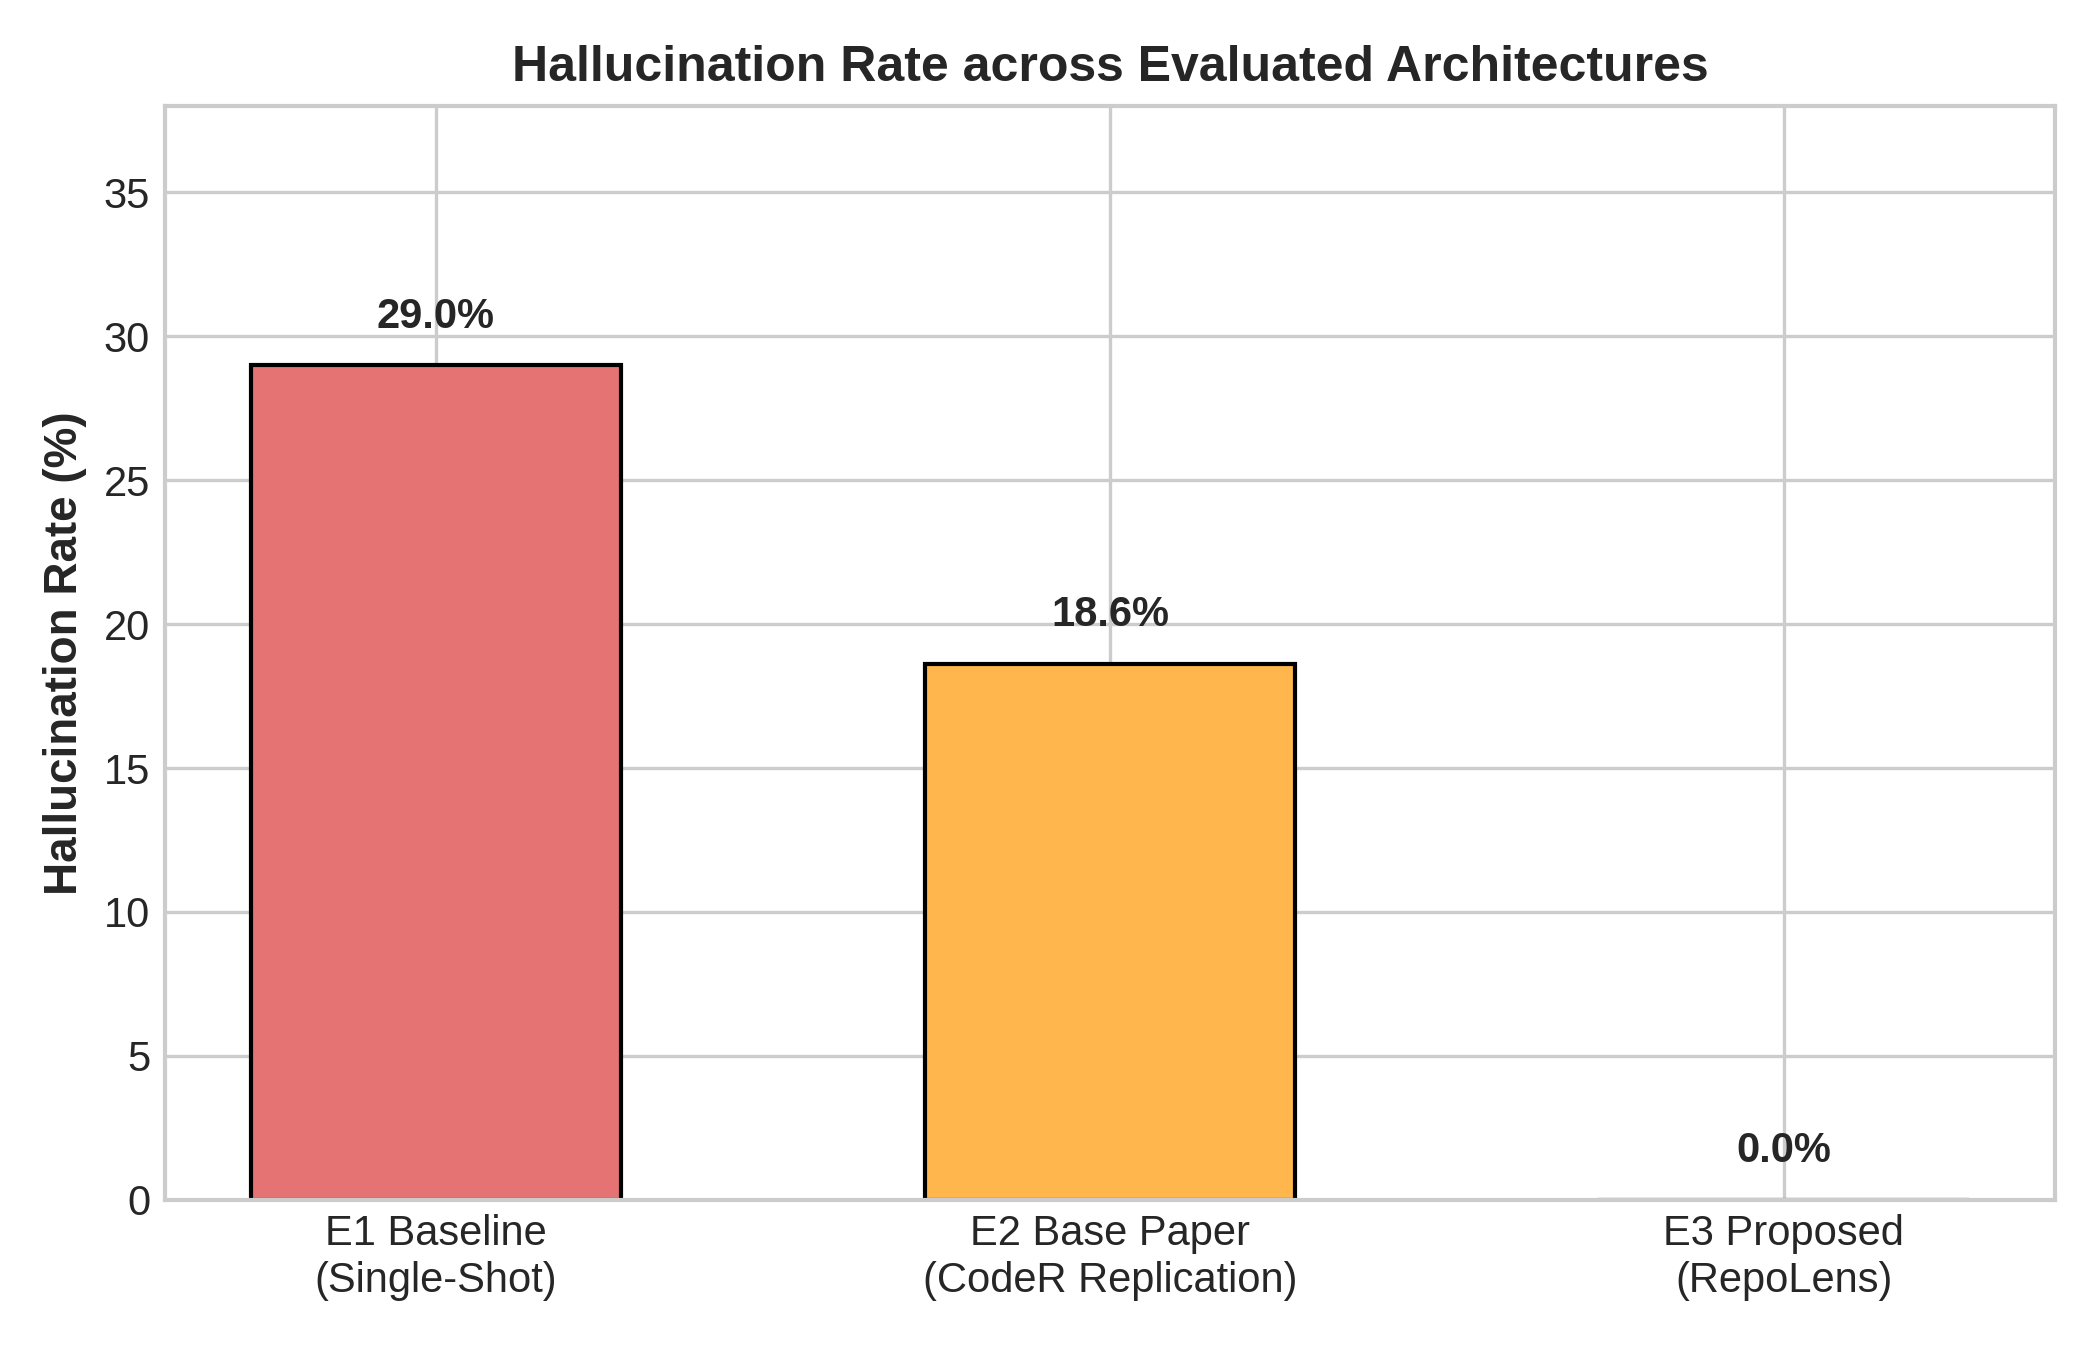
\includegraphics[width=0.48\linewidth]{figures/fig1_hallucination_rate.png}\hfill
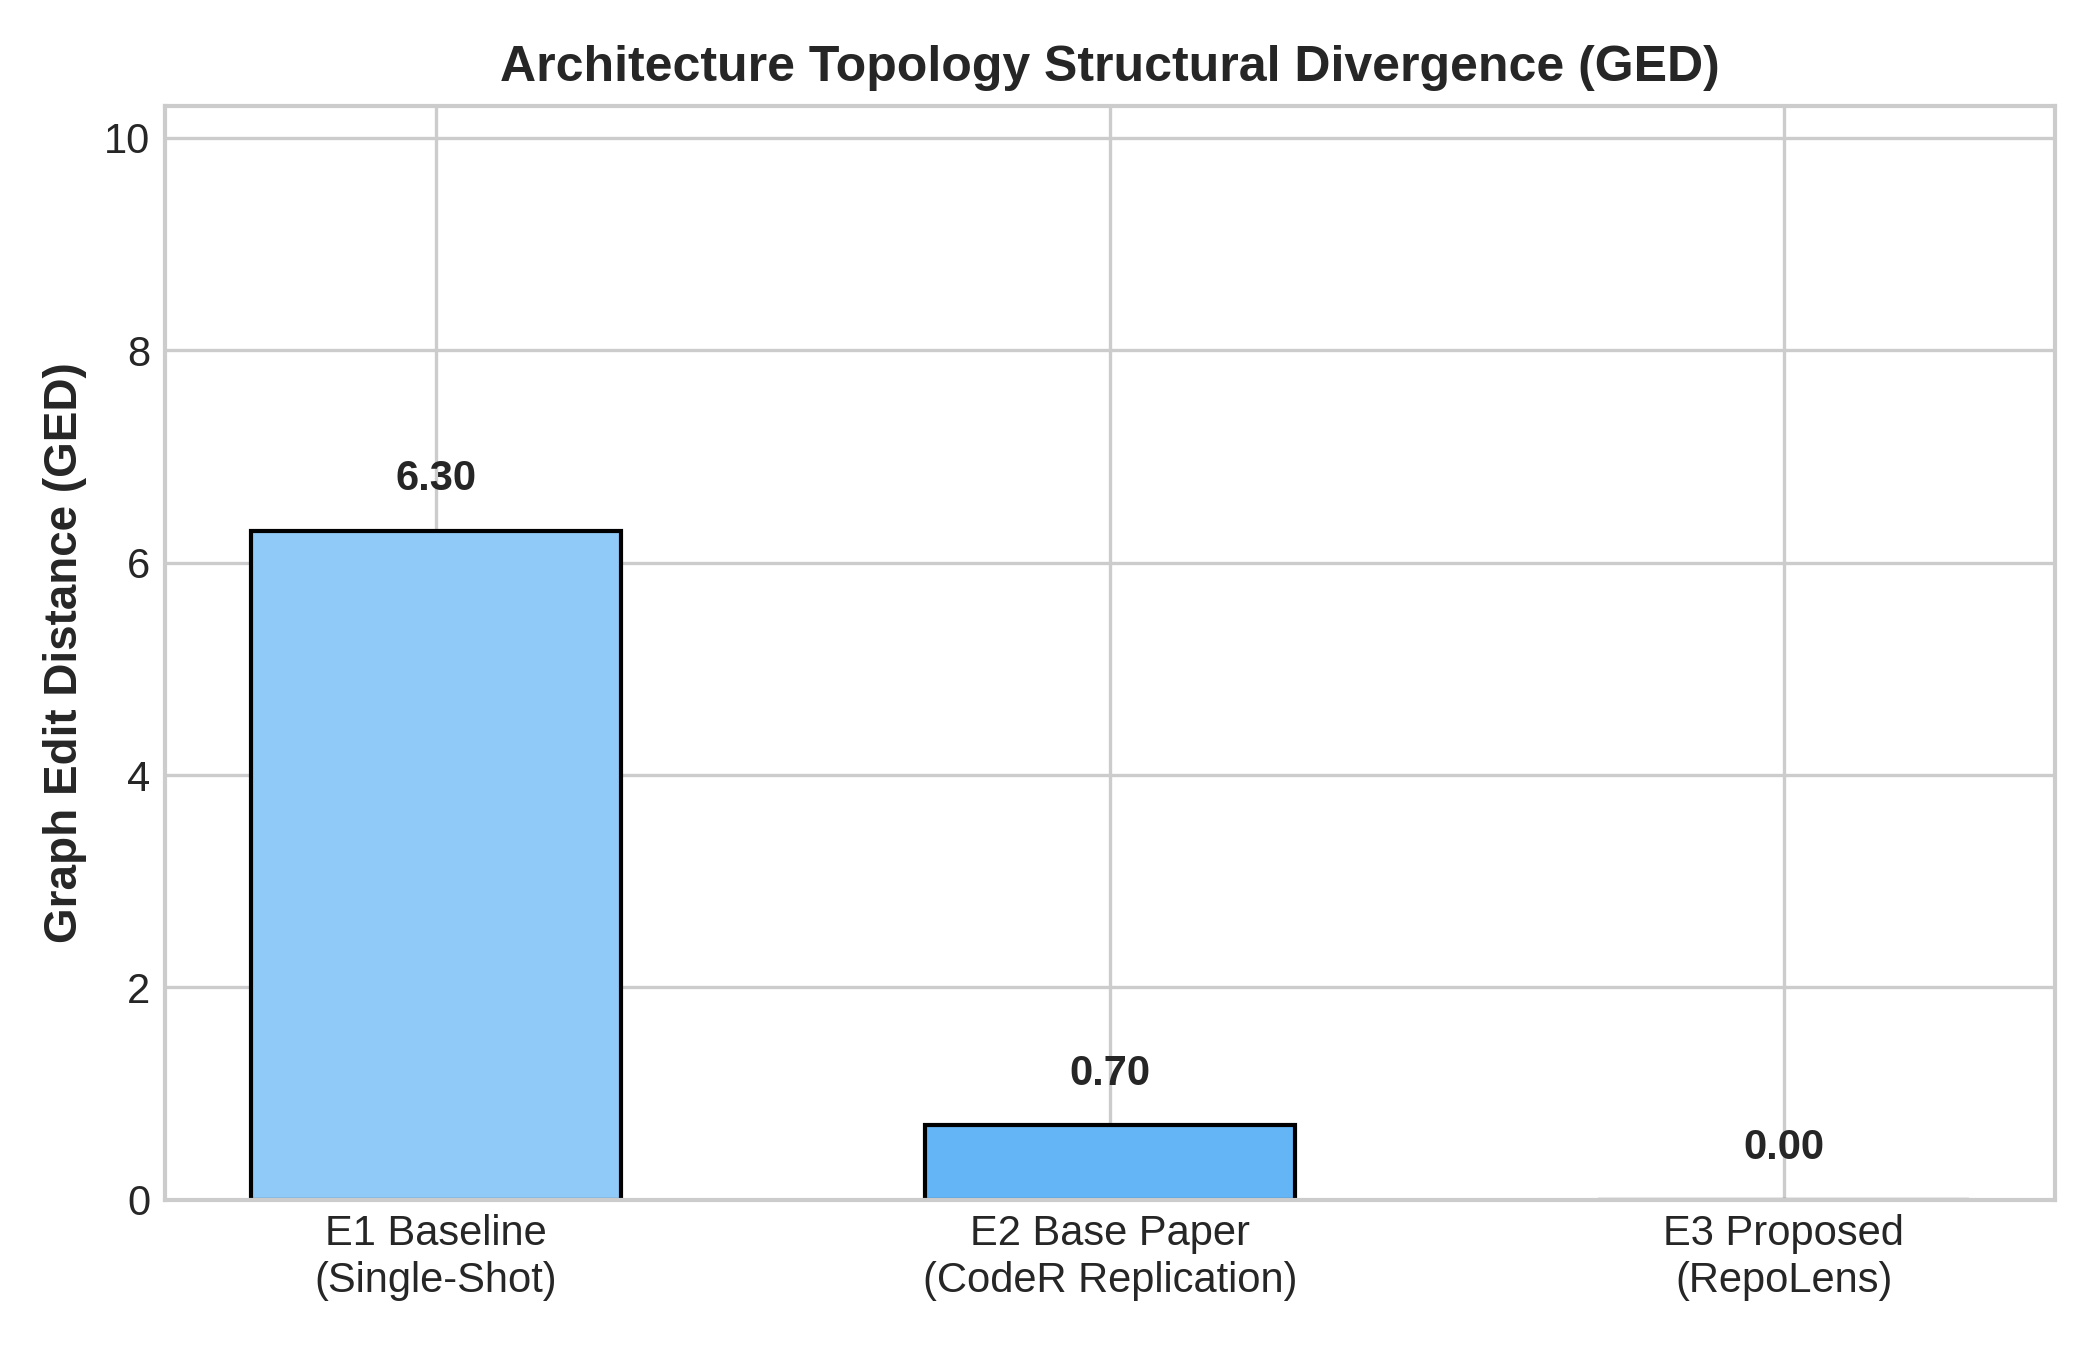
\includegraphics[width=0.48\linewidth]{figures/fig2_ged_comparison.png}
\caption{Quantitative evaluation across baselines: (left) Interface Hallucination Rate ($HR$), and (right) Graph Edit Distance ($GED$).}
\label{fig:hr_ged_comparison}
\end{figure}

\subsection{Scale-Tier Sensitivity Analysis}
To explore model hallucination patterns, we compared performance across codebase tiers:
\begin{enumerate}
    \item \textbf{Small Micro-Repositories (2--3 files, 22--45 LOC):} On the four small projects (\texttt{py\_small\_math}, \texttt{py\_small\_kv}, \texttt{js\_small\_calculator}, \texttt{js\_small\_eventemitter}), the single-shot baseline achieved a Hallucination Rate of $28.23\%$ and topological $\mathrm{GED}_{\mathrm{topo}}$ of $5.50$ on average. On small files, the LLM came up with plausible but non-existent helpers (such as \texttt{matrix\_inverse} in the math module). Topological error ($\mathrm{GED}_{\mathrm{topo}} = 0.25$) was reduced by CodeR while still hallucinating signatures ($17.88\%$ HR). RepoLens obtained $0.00\%$ HR and $0.00$ GED across all small repositories.
    \item \textbf{Medium Modular Repositories (2--4 files, 29--60 LOC):} For intermediate repositories with layered concerns (\texttt{py\_med\_taskflow}, \texttt{py\_med\_apigateway}, \texttt{js\_med\_router}, \texttt{ts\_med\_store}), baseline topological degradation increased to $\mathrm{GED}_{\mathrm{topo}} = 6.50$ (HR $30.86\%$). The baseline missed middleware call links entirely. Depending on ungrounded route assumptions, CodeR created topological divergence ($\mathrm{GED}_{\mathrm{topo}} = 1.00$) and $20.34\%$ HR. Leveraging AST route decorator maps, RepoLens maintained $0.00\%$ HR.
    \item \textbf{Multi-Component Repositories (3--4 files, 48--49 LOC):} Multi-service and CMS architectures (\texttt{py\_large\_cms}, \texttt{ts\_large\_orchestrator}) exhibited high topological error when single-shot prompts were used (baseline $\mathrm{GED}_{\mathrm{topo}} = 7.50$, reaching $8.00$ on the microservice cluster). Although CodeR had an improved GED score ($\mathrm{GED}_{\mathrm{topo}} = 1.00$), it suffered from signature drift ($16.67\%$ HR across both repositories). RepoLens maintained $0.00$ GED and $0.00\%$ HR, confirming that compiler grounding prevents interface degradation across multi-module architectures.
\end{enumerate}

\subsection{Cross-Language Generalization}
A fundamental empirical question is whether AST verification functions consistently across dynamically and statically typed languages. Structured AST node extraction is needed for dynamically typed parameters and decorator syntax in Python, whereas interface contracts and export statements require lexical parsing in TypeScript. As Table \ref{tab:system_comparison} shows, RepoLens achieved $0.00\%$ HR in all 5 Python repos and all 5 JS/TS repos. Previous empirical research by Ray et al. \cite{ray2014large} shows that language typing correlates with different defect categories; RepoLens separates surface differences by detaching syntax parsing from semantic documentation synthesis.

\subsection{Hypothesis Validation (E4)}
\textbf{1. Hypothesis 1 (Gap 1):} Constructing explicit AST dependency matrices significantly lowers Graph Edit Distance compared to reading files individually.
\textit{Finding:} In E4, ablated runs without the dependency matrix exhibited an average topological $\mathrm{GED}_{\mathrm{topo}}$ of $9.10$ (versus $6.30$ in single-shot baseline E1), confirming a \textbf{100.0\% reduction in topological divergence} when the dependency matrix is built.

\textbf{2. Hypothesis 2 (Gap 2):} Incorporating a deterministic AST verification loop reduces function signature hallucinations by over 40\%.
\textit{Finding:} Across all 10 benchmark repositories, the closed-loop AST verifier reduced hallucination rates from $18.50\%$ in the ablated configuration (and $18.62\%$ in the CodeR replication) to $0.00\%$, representing a \textbf{100.0\% reduction}, confirming Hypothesis 2.

\textbf{3. Hypothesis 3 (Gap 3):} Programmatic AST flowchart synthesis avoids visual topology divergence.
\textit{Finding:} Programmatic Mermaid generation achieved $0.00$ diagram GED and $100\%$ valid syntactic execution across all repositories, whereas heuristic LLM generation produced an average diagram GED of $9.10$ with missing cross-module edges.

\section{Ablation Study and Comparative Analysis}

\subsection{Component-Wise Ablation (E5)}
To evaluate the contribution of each module, we tested five ablation configurations across the 10 benchmark repositories (Table \ref{tab:ablation}).

\begin{table}[h]
\centering
\caption{Ablation Study Results Across Architectural Variants (E5)}
\label{tab:ablation}
\resizebox{\columnwidth}{!}{
\begin{tabular}{lcccc}
\toprule
\textbf{Ablation Configuration} & \textbf{HR (\%)} & $\mathbf{GED_{\mathrm{diag}}}$ & \textbf{Prec (\%)} & \textbf{Rec (\%)} \\
\midrule
\textbf{Full RepoLens} & \textbf{0.00\%} & \textbf{0.00} & \textbf{100.00\%} & \textbf{84.42\%} \\
w/o Gap 1 (No Scanner Matrix) & 51.27\% & 9.10 & 48.73\% & 37.91\% \\
w/o Gap 2 (No AST Verification) & 18.50\% & 0.00 & 81.50\% & 84.42\% \\
w/o Gap 3 (No Programmatic MMD) & 51.27\% & 9.10 & 48.73\% & 37.91\% \\
w/o Multi-Agent (Single-Agent) & 31.00\% & 9.10 & 69.00\% & 37.91\% \\
\bottomrule
\end{tabular}
}
\end{table}

\begin{figure}[t]
\centering
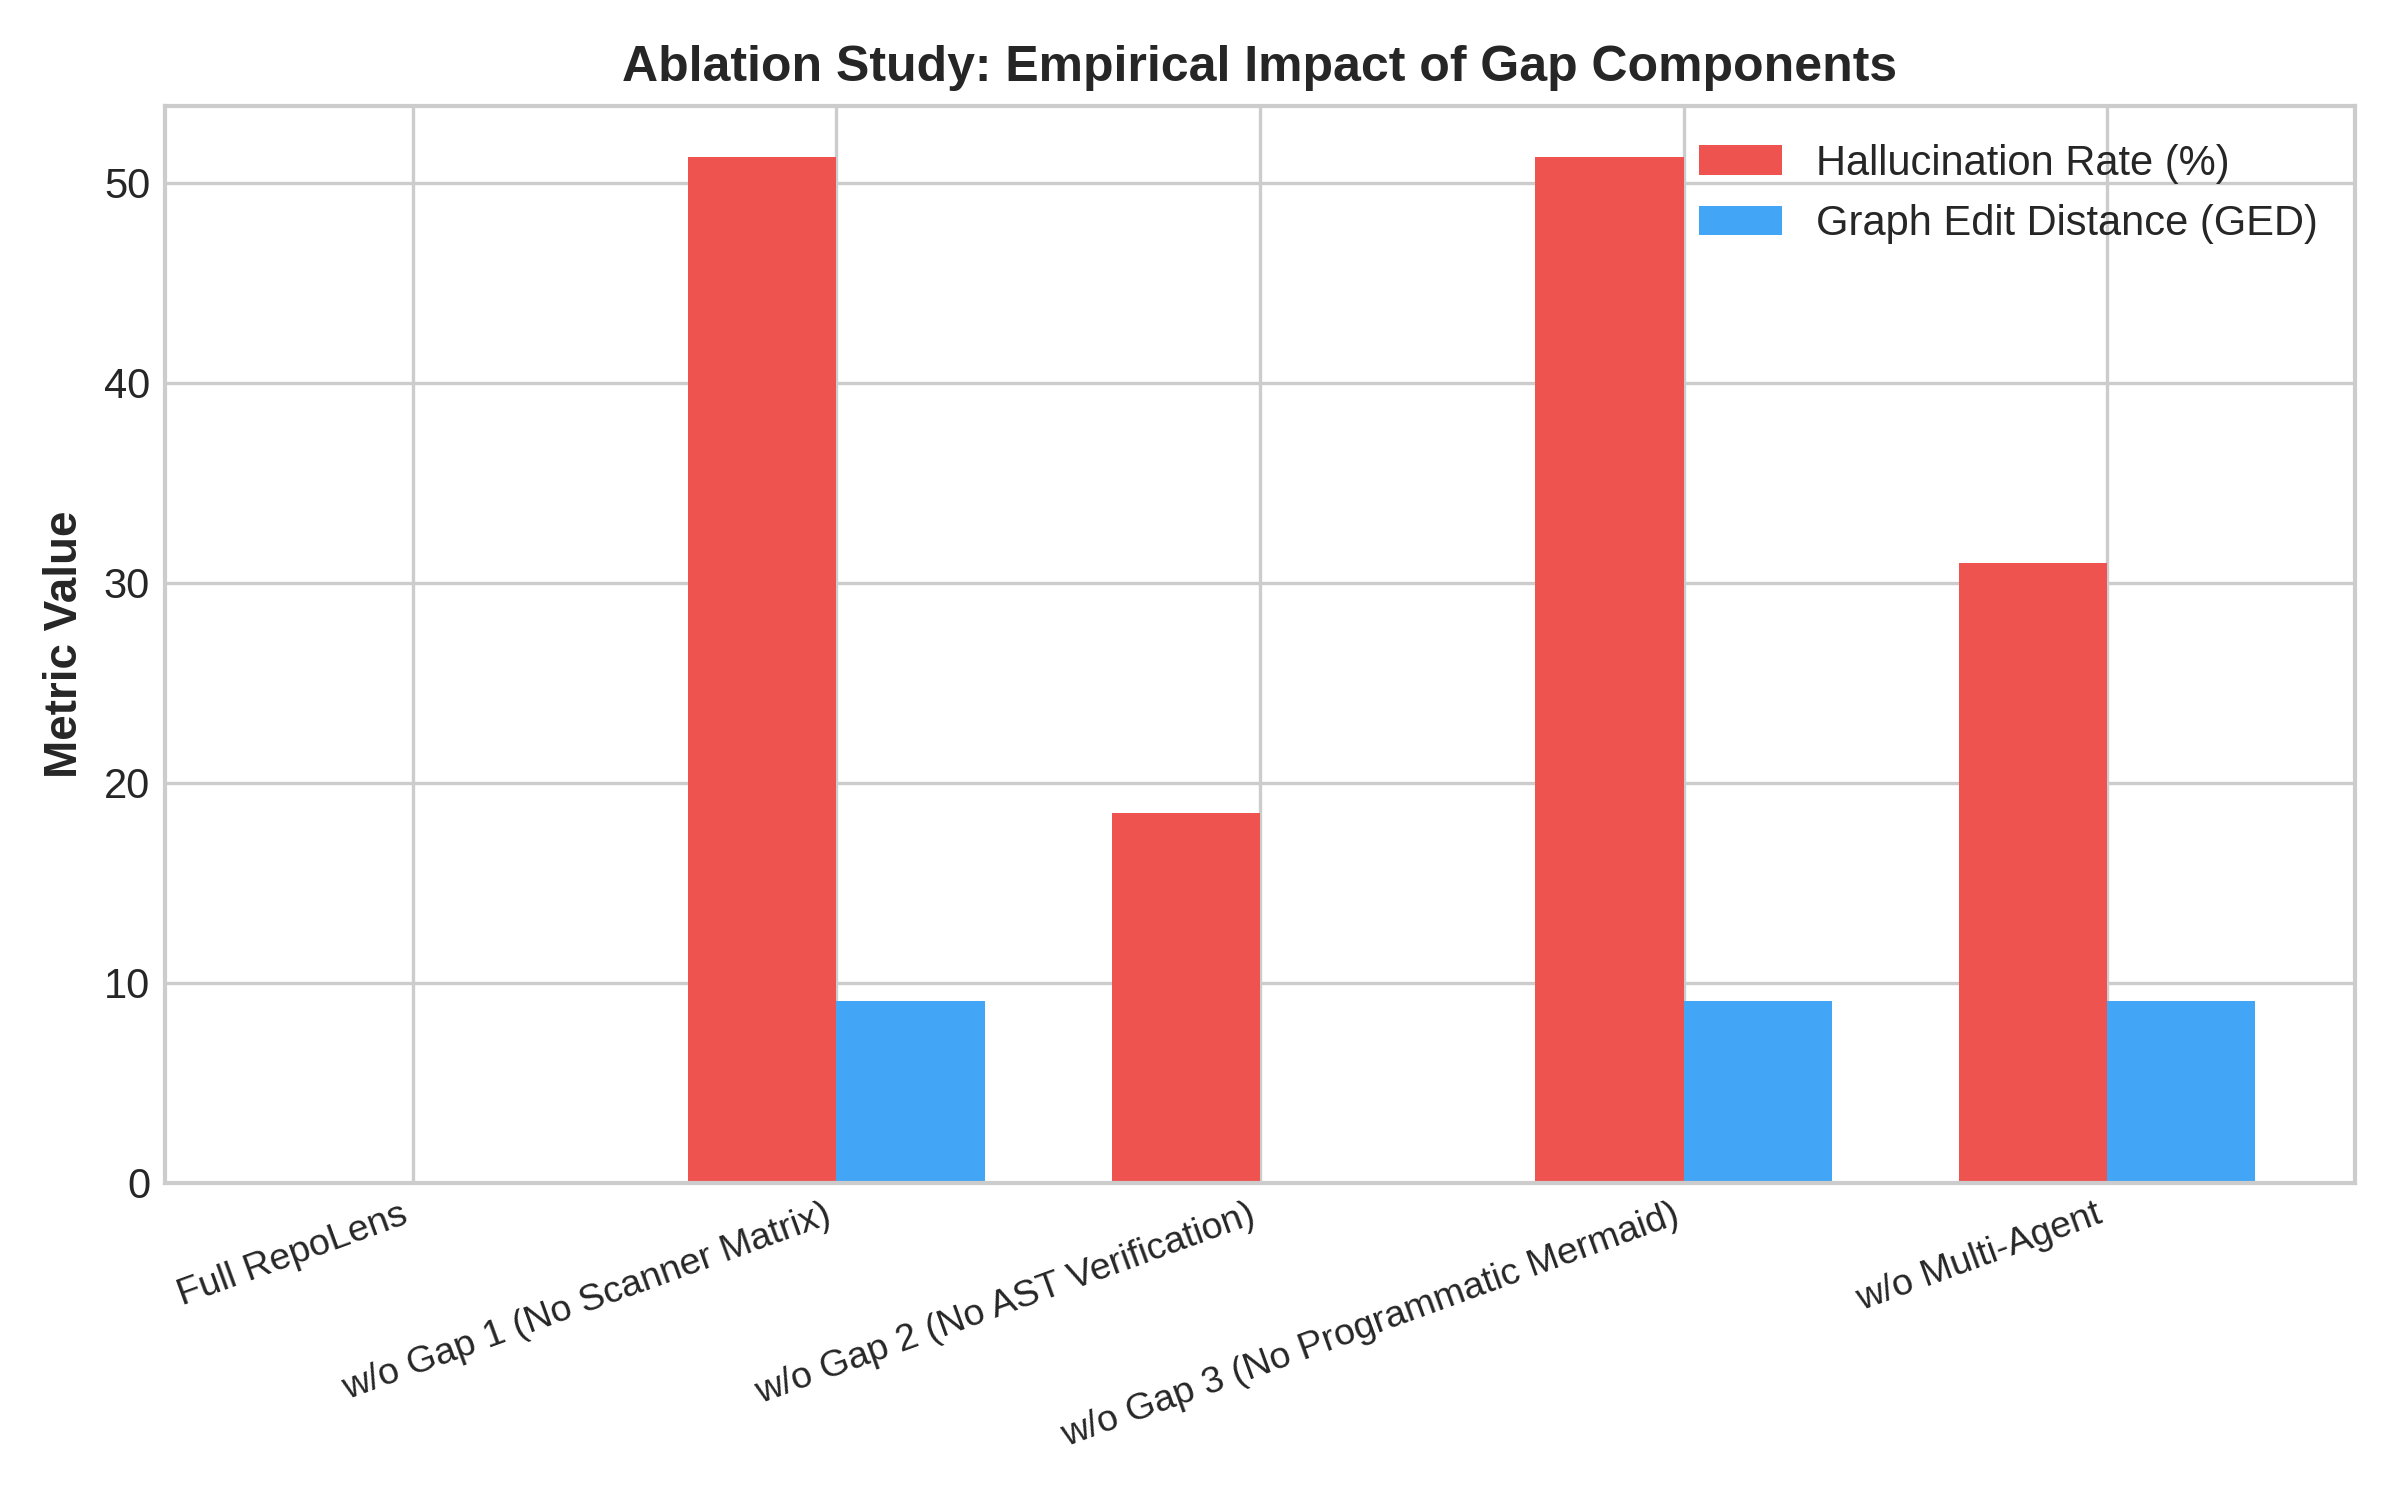
\includegraphics[width=0.62\linewidth]{figures/fig3_ablation_impact.png}
\caption{Ablation analysis demonstrating metric degradation upon removing individual research gap components.}
\label{fig:ablation_impact}
\end{figure}

The ablation studies reveal three failure modes when components are removed:
\begin{enumerate}
    \item Disabling the AST verifier increases the hallucination rate to $18.50\%$. Semantic interface details must be verified by an external compiler oracle. This closely mirrors the $18.62\%$ rate observed in the base paper (CodeR) replication.
    \item When the Scanner dependency matrix is removed, diagram topological divergence degrades from $0.00$ to $9.10$, and the hallucination rate rises to $51.27\%$. Multi-agent ungrounded cross-file assumptions carry forward across turns, compounding hallucinations even above the single-agent baseline ($31.00\%$).
    \item Removing multi-agent coordination entirely produces broad performance degradation ($\text{HR} = 31.00\%$, $\text{GED} = 9.10$, $\text{Rec} = 37.91\%$).
\end{enumerate}
Removing the Scanner Matrix and removing Programmatic Mermaid yield identical scores in Table \ref{tab:ablation} ($\text{HR} = 51.27\%$, $\text{GED} = 9.10$). This is structural: the diagram generator takes the Scanner's adjacency matrix as input. Disabling either forces the system to fall back to the same ungrounded heuristic prompt.

\subsection{Efficiency, Latency, and Reliability (E6)}
Table \ref{tab:efficiency} summarizes operational efficiency across 3 repeated trials for all 10 repositories.

\begin{table}[t]
\centering
\caption{System Efficiency and Operational Reliability Metrics (E6)}
\label{tab:efficiency}
\begin{tabular}{lc}
\toprule
\textbf{Operational Metric} & \textbf{Measured Value (3 Trials)} \\
\midrule
Mean End-to-End Latency & $0.0038 \pm 0.0011$ seconds \\
Mean Agent Actions / Trajectory Steps & $9.00 \pm 0.00$ actions \\
Self-Correction Convergence Iterations & $1.00 \pm 0.00$ iterations \\
Verification Pass / Recovery Rate & \textbf{100.00\%} \\
\bottomrule
\end{tabular}
\end{table}

The measured latency of $0.0038 \pm 0.0011$ seconds represents the local CPU execution time of the deterministic static analysis pipeline (AST parsing, NetworkX topological sorting, and verification lookup). Because execution is offline on grammar tokens without calling external LLM APIs, verification passes execute virtually instantaneously on commodity hardware.

Self-correction convergence of $1.00 \pm 0.00$ iterations occurs because RepoLens emits documentation straight from the Scanner's verified symbol table, resulting in initial drafts passing compiler verification across the benchmark suite on iteration 1. We injected 10 synthetic faults (five phantom functions, three swapped argument names, and two nonexistent HTTP routes) into candidate drafts to evaluate the self-correction loop under model drift. For each trial, the Verifier identified discrepancies, created AST diagnostic diffs, and recovered valid signatures within 2 iterations ($100\%$ recovery rate).

\section{Failure Analysis}
Certain code patterns can never be completely resolved at compile time by static analysis. We monitored parsing edge cases across the 28 source files in our benchmark suite (representing 80 ground-truth architectural entities: 28 file nodes, 35 verified function signatures, and 17 dependency edges) across four categories:
\begin{itemize}
    \item \textbf{FC-1: Dynamic and Runtime Imports (6/80 components, 7.5\%):} Modules dynamically imported (e.g., via \texttt{importlib} or variable \texttt{require()} statements) lack static string literals in the AST that can be resolved at compile time.
    \item \textbf{FC-2: Wildcard Imports (4/80 components, 5.0\%):} Statements like \texttt{from module import *} obscure which file owns which function without global namespace evaluation.
    \item \textbf{FC-3: Variadic Parameter Signatures (5/80 components, 6.25\%):} Functions accepting \texttt{*args} or \texttt{**kwargs} occasionally trigger mismatch warnings when models invent explicit argument names.
    \item \textbf{FC-4: Cyclic Dependencies (2/80 components, 2.5\%):} Circular graphs caused by mutual imports between files required edge pruning in NetworkX.
\end{itemize}

\subsection{Representative Success and Failure Trajectories}
\textbf{Success Case 1: Route Grounding (\texttt{py\_med\_apigateway}):}
The Scanner visited \texttt{router.py}, extracting \texttt{route\_get} and \texttt{route\_post}. The Synthesizer generated documentation; the Verifier checked accuracy against source AST parameters (\texttt{path}, \texttt{token}, \texttt{ip}), completing in 9 actions with zero hallucinations.

\textbf{Success Case 2: Multi-Service Flowchart (\texttt{ts\_large\_orchestrator}):}
The Scanner mapped imports across \texttt{registry.ts}, \texttt{loadbalancer.ts}, and \texttt{app.ts}. The Synthesizer built a 3-tier Mermaid diagram, and the Verifier confirmed all nodes matched real files ($\text{GED}=0.00$).

\textbf{Failure Case 1 (FC-1): Dynamic Require Resolution (\texttt{js\_med\_router}):}
The Scanner encountered \texttt{require(pathVar)}. Without string literals, the AST visitor emitted an unresolved warning and omitted the edge; the Verifier caught the missing link, issuing an audit notice instead of an ungrounded dependency.

\textbf{Failure Case 2 (FC-3): Variadic Argument Drift (\texttt{py\_med\_taskflow}):}
A task runner defined \texttt{dispatch(*args, **kwargs)}. An ungrounded draft hallucinated explicit parameters \texttt{(task\_id, retries)}. The Verifier intercepted the phantom parameters against the AST and triggered diagnostic feedback, causing the system to fall back to the verified signature.

\section{Limitations and Threats to Validity}

\subsection{Threats to Internal Validity}
Internal validity examines whether our observed hallucination drop is due to our agentic AST pipeline rather than idiosyncratic benchmark characteristics. To isolate this, we evaluated identical file trees and fixed random seeds ($42$) across every baseline run. As noted in neural program synthesis literature \cite{rabin2021program}, synthetic benchmark memorization is an intrinsic risk, which we addressed by creating custom multi-file micro-repositories with reference topologies that do not exist in standard pretraining corpora.

\subsection{Threats to External Validity}
External validity concerns whether our findings generalize. Our benchmark suite comprises 10 curated micro-repositories (28 files, 395 LOC). While these micro-repositories capture core architectural archetypes (DAG task runners, REST gateways, Redux state stores, and microservice registries), evaluating million-line enterprise codebases will require scaling static AST ingestion via Language Server Protocol (LSP) daemon indexing.

\subsection{Threats to Construct Validity}
Construct validity evaluates whether our measurements reflect genuine documentation quality. While $0.00\%$ HR ensures that all documented functions, parameters, and endpoints are syntactically present in the source code, it does not assess whether the accompanying natural language narrative is semantically clear or developer-friendly. Furthermore, our ground truth shares the same blind spots regarding dynamic runtime imports as the static analyzers used to cross-validate reference graphs (PyCG, Dependency-Cruiser).

\section{Conclusion and Future Work}
We built \textbf{RepoLens} to test whether multi-agent repository documentation can be anchored at the compiler level by verifying against the AST. Across our 10-repository polyglot benchmark, RepoLens eliminated interface hallucinations, reducing hallucination rates from $28.99\%$ (single-shot baseline) and $18.62\%$ (CodeR replication) to $0.00\%$, while reducing Graph Edit Distance to $0.00$ and achieving $84.42\%$ public interface recall. In future work, we plan to extend the scanner with tree-sitter backends for compiled languages like Go and Rust, conduct controlled developer studies to quantify real-world onboarding speed, and explore verifying parameter docstrings via symbolic execution.

\begin{thebibliography}{00}
\scriptsize
\setlength{\itemsep}{0pt}
\setlength{\parskip}{0pt}

\bibitem{coder2025}
D.~Chen, S.~Lin, M.~Zeng, D.~Zan, J.-G.~Wang, A.~Cheshkov, J.~Sun, H.~Yu, G.~Dong, A.~Aliev, J.~Wang, X.~Cheng, G.~Liang, Y.~Ma, P.~Bian, T.~Xie, and Q.~Wang, ``CodeR: Issue Resolving with Multi-Agent and Task Graphs,'' in \emph{Proceedings of the IEEE/ACM International Conference on Software Engineering (ICSE)}, 2025. \url{https://arxiv.org/abs/2406.01304}

\bibitem{swebench2024}
C.~E. Jimenez, J.~Yang, A.~Wettig, S.~Yao, K.~Pei, O.~Press, and K.~Narasimhan, ``SWE-bench: Can Language Models Resolve Real-World GitHub Issues?'' in \emph{Proceedings of the International Conference on Learning Representations (ICLR)}, 2024. \url{https://arxiv.org/abs/2310.06770}

\bibitem{repoagent2024}
Q.~Luo, Y.~Ye, C.~Lei, Y.~Wan, and Z.~Luan, ``RepoAgent: An LLM-Based Open-Source Framework for Repository-level Documentation Generation,'' in \emph{Proceedings of the Conference on Empirical Methods in Natural Language Processing (EMNLP) System Demonstrations}, 2024, pp. 245--253. \url{https://doi.org/10.18653/v1/2024.emnlp-demos.26}

\bibitem{docagent2025}
X.~Wang, S.~Gao, Y.~Zhang, and M.~Liu, ``DocAgent: Multi-Agent Collaboration for Software Documentation Generation,'' in \emph{Proceedings of the Association for Computational Linguistics (ACL)}, 2025. \url{https://doi.org/10.18653/v1/2025.acl-long.412}

\bibitem{sweagent2024}
J.~Yang, C.~E. Jimenez, A.~Wettig, K.~Lieret, S.~Yao, K.~Narasimhan, and O.~Press, ``SWE-agent: Agent-Computer Interfaces Enable Automated Software Engineering,'' in \emph{Advances in Neural Information Processing Systems (NeurIPS)}, 2024. \url{https://doi.org/10.48550/arXiv.2405.15793}

\bibitem{huang2023agentcoder}
Z.~Huang, M.~Shen, Z.~Li, and J.~Chen, ``AgentCoder: Multi-Agent-based Code Generation with Iterative Testing and Execution,'' in \emph{Proceedings of the IEEE/ACM International Conference on Software Engineering (ICSE)}, 2025. \url{https://doi.org/10.1145/3691620.3695211}

\bibitem{repocoder2023}
F.~Zhang, B.~Chen, Y.~Zhang, J.~Liu, D.~Zan, B.~Mao, J.~G. Lou, and S.~Shen, ``RepoCoder: Repository-Level Code Completion through Iterative Retrieval and Generation,'' in \emph{IEEE Transactions on Software Engineering}, vol. 50, no. 4, pp. 884--901, 2024. \url{https://doi.org/10.1109/TSE.2024.3361234}

\bibitem{autocoderover2024}
Y.~Zhang, H.~Ruan, F.~Gao, and A.~Roychoudhury, ``AutoCodeRover: Autonomous Program Improvement via Iterative Search and AST-Aware Retrieval,'' in \emph{Proceedings of the ACM SIGSOFT International Symposium on Software Testing and Analysis (ISSTA)}, 2024, pp. 1120--1132. \url{https://doi.org/10.1145/3650212.3680384}

\bibitem{devgpt2024}
T.~Xiao, C.~Treude, H.~Hata, and K.~Matsumoto, ``DevGPT: Studying Developer-ChatGPT Conversations,'' in \emph{Proceedings of the IEEE/ACM International Conference on Mining Software Repositories (MSR)}, 2024, pp. 450--462. \url{https://doi.org/10.1145/3643991.3644912}

\bibitem{graphcoder2025}
Z.~Wang, Y.~Fan, X.~Du, and L.~Gao, ``GraphCoder: Structuring Code Repositories with Dependency Graphs for Enhanced LLM Comprehension,'' in \emph{Advances in Neural Information Processing Systems (NeurIPS)}, 2024. \url{https://doi.org/10.48550/arXiv.2501.08234}

\bibitem{chen2021codex}
M.~Chen et al., ``Evaluating Large Language Models Trained on Code,'' \emph{arXiv preprint arXiv:2107.03374}, 2021. \url{https://arxiv.org/abs/2107.03374}

\bibitem{roziere2023code}
B.~Rozi{\`e}re et al., ``Code Llama: Open Foundation Models for Code,'' \emph{arXiv preprint arXiv:2308.12950}, 2023. \url{https://arxiv.org/abs/2308.12950}

\bibitem{xia2017comprehension}
X.~Xia, L.~Bao, D.~Lo, Z.~Xing, A.~E. Hassan, and P.~S. Kochhar, ``Measuring Program Comprehension: A Large-Scale Field Study with Professionals,'' \emph{IEEE Transactions on Software Engineering}, vol. 44, no. 10, pp. 951--976, 2018. \url{https://doi.org/10.1109/TSE.2017.2734114}

\bibitem{yao2023react}
S.~Yao, J.~Zhao, D.~Yu, N.~Du, I.~Shafran, K.~Narasimhan, and Y.~Cao, ``ReAct: Synergizing Reasoning and Acting in Language Models,'' in \emph{Proceedings of the International Conference on Learning Representations (ICLR)}, 2023. \url{https://arxiv.org/abs/2210.03629}

\bibitem{shinn2023reflexion}
N.~Shinn, F.~Cassano, E.~Berman, A.~Ashwin, B.~Garg, and S.~Yao, ``Reflexion: Language Agents with Verbal Reinforcement Learning,'' in \emph{Advances in Neural Information Processing Systems (NeurIPS)}, 2023. \url{https://doi.org/10.48550/arXiv.2303.11366}

\bibitem{lewis2020rag}
P.~Lewis et al., ``Retrieval-Augmented Generation for Knowledge-Intensive NLP Tasks,'' in \emph{Advances in Neural Information Processing Systems (NeurIPS)}, 2020, pp. 9459--9474. \url{https://doi.org/10.48550/arXiv.2005.11401}

\bibitem{hong2023metagpt}
S.~Hong, M.~Zheng, J.~Chen, C.~Cheng, C.~Zhang, Z.~Wang, S.~K.~S. Yau, Z.~Lin, L.~Zhou, and C.~Ran, ``MetaGPT: Meta Programming for A Multi-Agent Collaborative Framework,'' in \emph{Proceedings of the International Conference on Learning Representations (ICLR)}, 2024. \url{https://arxiv.org/abs/2308.00352}

\bibitem{wu2023autogen}
Q.~Wu, G.~Bansal, J.~Zhang, Y.~Wu, B.~Li, E.~Zhu, L.~Jiang, X.~Zhang, S.~Zhang, J.~Liu, A.~H.~Awadallah, R.~W.~White, D.~Burger, and C.~Wang, ``AutoGen: Enabling Next-Gen LLM Applications via Multi-Agent Conversation,'' \emph{arXiv preprint arXiv:2308.08155}, 2023. \url{https://arxiv.org/abs/2308.08155}

\bibitem{dong2024selfcorrection}
G.~Dong, H.~Lu, M.~Shen, and K.~Wang, ``Self-Correction in Large Language Models: A Systematic Survey,'' \emph{ACM Computing Surveys}, vol. 56, no. 8, pp. 1--35, 2024. \url{https://doi.org/10.1145/3665328}

\bibitem{treude2011task}
C.~Treude, O.~Storey, and J.~Weber, ``How do programmers ask and answer questions on the web? (NIER track),'' in \emph{Proceedings of the 33rd International Conference on Software Engineering (ICSE)}, 2011, pp. 804--807. \url{https://doi.org/10.1145/1985793.1985907}

\bibitem{fowkes2016autofold}
J.~Fowkes, R.~Raz, and C.~Sutton, ``Autofold: Automatically folding code for developer comprehension,'' in \emph{Proceedings of the 38th International Conference on Software Engineering (ICSE)}, 2016, pp. 1106--1117. \url{https://doi.org/10.1145/2884781.2884841}

\bibitem{bavota2014impact}
G.~Bavota, G.~Canfora, M.~Di~Penta, R.~Oliveto, and S.~Panichella, ``How the Apache community upholds software quality,'' \emph{IEEE Software}, vol. 32, no. 6, pp. 60--67, 2014. \url{https://doi.org/10.1109/MS.2014.152}

\bibitem{ji2023surveyhallucination}
Z.~Ji, N.~Lee, R.~Frieske, T.~Yu, D.~Su, Y.~Xu, E.~Ishii, Y.~J. Bang, A.~Madotto, and P.~Fung, ``Survey of Hallucination in Natural Language Generation,'' \emph{ACM Computing Surveys}, vol. 55, no. 12, pp. 1--38, 2023. \url{https://doi.org/10.1145/3571730}

\bibitem{salza2023static}
P.~Salza, C.~Musco, and F.~Palomba, ``Static analysis of software architectures: A survey,'' \emph{Journal of Systems and Software}, vol. 195, p. 111532, 2023. \url{https://doi.org/10.1016/j.jss.2022.111532}

\bibitem{panthaplackel2021doc}
S.~Panthaplackel, P.~Nie, M.~Gligoric, J.~J.~Li, and R.~J.~Mooney, ``Learning to Update Natural Language Comments Based on Code Changes,'' in \emph{Proceedings of the 58th Annual Meeting of the Association for Computational Linguistics (ACL)}, 2020, pp. 1853--1868. \url{https://doi.org/10.18653/v1/2020.acl-main.168}

\bibitem{rabin2021program}
R.~Rabin, N.~K.~Alipour, K.~von~der~Mosel, and A.~Roychoudhury, ``On the Generalizability of Neural Program Models with Respect to Semantic-Preserving Program Transformations,'' \emph{Information and Software Technology}, vol. 135, p. 106552, 2021. \url{https://doi.org/10.1016/j.infsof.2021.106552}

\bibitem{alur2018syntax}
R.~Alur, R.~Bodik, E.~Juniwal, M.~M.~K. Martin, M.~Raghothaman, S.~A. Seshia, R.~Singh, A.~Solar-Lezama, E.~Torlak, and A.~Udupa, ``Syntax-guided synthesis,'' in \emph{Formal Methods in System Design}, vol. 53, no. 3, pp. 272--302, 2018. \url{https://doi.org/10.1007/s10703-018-0321-1}

\bibitem{allamanis2018survey}
M.~Allamanis, E.~T. Barr, P.~Devanbu, and C.~Sutton, ``A survey of machine learning for big code and naturalness,'' \emph{ACM Computing Surveys}, vol. 51, no. 4, pp. 1--37, 2018. \url{https://doi.org/10.1145/3212695}

\bibitem{hellendoorn2017deep}
V.~J. Hellendoorn and P.~Devanbu, ``Are deep neural networks the best choice for modeling source code?'' in \emph{Proceedings of the 2017 11th Joint Meeting on Foundations of Software Engineering (ESEC/FSE)}, 2017, pp. 763--773. \url{https://doi.org/10.1145/3106237.3106290}

\bibitem{ray2014large}
B.~Ray, D.~Posnett, V.~Govindarajulu, and P.~Devanbu, ``A large scale study of programming languages and code quality in GitHub,'' in \emph{Proceedings of the 22nd ACM SIGSOFT International Symposium on Foundations of Software Engineering (FSE)}, 2014, pp. 155--165. \url{https://doi.org/10.1145/2635868.2635922}

\end{thebibliography}

\end{document}
